\section{Background}\label{sec:background}
This section introduces biodiversity and how it is measured in Section~\ref{subsec:biodiversity}. Section~\ref{subsec:modeling-definition} provides a mathematical framework for understanding top-down modeling approaches, so we can use them for predicting community-level biodiversity metrics. In Section~\ref{}This background section provides the necessary context for understanding the methods and results presented in this thesis. It also highlights the differences between the modeling approaches as well as the different assumptions and limitations of these models. 
\subsection{Biodiversity and community-level biodiversity metrics}\label{subsec:biodiversity}
%here we want to also talk about biodiversity metrics in alpha diversity and how they are calculated and the different types of metrics that exist. 
%section here about biodiversity and taxa in general and how taxa hierarchy and how we will measure it. Should include a discussion of the different metrics for measuring biodiversity and how they are calculated. Also include a discussion of the different types of taxa and how they are classified. This section will set the stage for the rest of the background and methods sections where we will discuss how to model biodiversity and the different types of models that have been developed for this purpose.

Biodiversity is a complex and multifaceted concept that encompasses the variety of life on Earth, including the diversity of species, genetic diversity within species, and the diversity of ecosystems \parencite{Stork2009}. Humanity has relied on biodiversity for survival for thousands of years as it provides us with food, materials, medicine, water security, and has a substantial impact on human health and well-being \parencite{gascon2015,naeem2016, brauman2020, kim2024}. Large losses of biodiversity would be catastrophic for humanity and ecosystems as it would lead to the loss of ecosystem functions, the collapse of food webs, adversely affect human health, degrade medicine production and discovery, and more \parencite{roe2018}. The rate of biodiversity loss is unprecedented, and we are quickly moving towards a sixth mass extinction \parencite{cowie2022}. To combat biodiversity loss effectively, conservation and ecological rehabilitation efforts require accurate, robust models that can predict biodiversity patterns, identify priority areas, and assess potential conservation outcomes \parencite{sinclair2010, pollock2020}.

To effectively predict biodiversity, it is crucial to have a clear understanding of how biodiversity data is collected and measured. Generally, biodiversity data is collected through field surveys, remote sensing, and citizen science initiatives and other monitoring schemes depending on what is being measured \parencite{proenca2017, beery2021,brun2024}. These approaches or protocols can provide data on species occurrences, abundances, and distributions across different spatial scales \parencite{proenca2017}. Common biodiversity datasets can be categorized by the type of species information they contain. Presence-only data record locations where a species has been observed, but do not provide information on confirmed absences. Presence-absence data record whether each species is present or absent at a site. Abundance data provide counts or estimates of the number of individuals of each species at a site. Once these raw data is collected, there are three broad categories of biodiversity metrics that are computed: alpha diversity, beta diversity, and gamma diversity. Alpha diversity refers to diversity within a site, such as the diversity within a specific community or ecosystem. Beta diversity refers to the diversity between different communities or ecosystems. Gamma diversity refers to the species diversity across communities or ecosystems within a larger region \parencite{andermann2022}. For the purposes of this thesis, we will focus on alpha diversity.

Common alpha diversity metrics include species richness, absolute abundance, relative abundance, Shannon index, arithmetic mean abundance, and geometric mean abundance \parencite{santini2017, beery2021}. Species richness is the most commonly used metric and simply counts the number of species in a given area \parencite{ferrier2006}. Species richness is a very popular metric because presence-absence data is the most common type of biodiversity data \parencite{ozkan_tumer_two_2026}. Absolute abundance measures the total number of individuals of each species at a site, and relative abundance measures the proportion of individuals of each species relative to the total number of individuals in a site \parencite{beery2021}. The Shannon index is another commonly used metric and combines species richness and evenness into a single metric and quantifies the uncertainty in predicting the species of an individual randomly selected from a community \parencite{beery2021}. Arithmetic mean abundance is the average abundance of species in a given area, and geometric mean abundance is the exponential of the average of the log abundances of species in a given area \parencite{santini2017}.

For the purposes of this thesis, it is beneficial to express these terms mathematically. Community-level biodiversity metrics are usually calculated at the site level. A site is a spatial sampling unit that is defined according to a sampling protocol. We define a site as \(r\), which is a spatial location, and within a biodiversity dataset there are \(n\) sites which make up the region of interest \(R = \{r_1, r_2, \ldots , r_n\}\). Across the entire region of interest \(R\) there is a set \(S\) of unique species that were observed, and \(s\) is a specific species, where \(s \in S\). Furthermore, let \(a_{s,r_i}\) be the abundance or count of individuals of species \(s\) at site \(r_i\).

The alpha diversity metrics used in this thesis are therefore defined at the site level as follows.

\noindent\textbf{Species richness.} Following Beery et al. \parencite{beery2021}, species richness is the number of unique species \(s\) at a given site \(r_i\) and can be expressed as:
\begin{equation}
SR_{r_i} = \sum_{s \in S} \mathbf{1}(a_{s,r_i} > 0),
\label{eq:species-richness-site}
\end{equation}
where \(\mathbf{1}(\cdot)\) is the indicator function that equals 1 if the condition is true and 0 otherwise.
For reference, regional species richness across \(R\) can be expressed as:
\begin{equation}
SR_R = \left|S\right|.
\label{eq:species-richness-regional}
\end{equation}

\noindent\textbf{Absolute abundance.} Absolute abundance is the total number of individuals across species \(s\) at a given site \(r_i\) and can be expressed as:
\begin{equation}
A_{r_i} = \sum_{s \in S} a_{s,r_i},
\label{eq:absolute-abundance}
\end{equation}
where \(a_{s,r_i}\) is the abundance or count of individuals of species \(s\) at site \(r_i\) \parencite{beery2021}, and \(a_{s,r_i} = 0\) if species \(s\) is not present at site \(r_i\).

\noindent\textbf{Relative abundance.} Relative abundance is the proportion of individuals of each species \(s\) relative to the total number of individuals at a given site \(r_i\) and can be expressed as:
\begin{equation}
p_{s,r_i} = \frac{a_{s,r_i}}{A_{r_i}},
\label{eq:relative-abundance}
\end{equation}
where \(a_{s,r_i}\) is the abundance or count of individuals of species \(s\) at site \(r_i\) and \(A_{r_i}\) is the total abundance of all species at site \(r_i\) \parencite{beery2021}. If \(a_{s,r_i} = 0\) then species \(s\) is not present at site \(r_i\), and \(p_{s,r_i} = 0\).

\noindent\textbf{Shannon index.} The Shannon index combines species richness and evenness into a single metric and quantifies the uncertainty in predicting the species of an individual randomly selected from a community. It can be expressed as:
\begin{equation}
H_{r_i} = -\sum_{s \in S} p_{s,r_i} \ln(p_{s,r_i}),
\label{eq:shannon-index}
\end{equation}
where \(p_{s,r_i}\)is the relative abundance of species \(s\) at site \(r_i\). If \(p_{s,r_i} = 0\), then that term is not include in the calculation. The interpretation of the Shannon index is that higher values of \(H_{r_i}\) indicate higher diversity \parencite{dusek2017}. 

\noindent\textbf{Arithmetic mean abundance.} Arithmetic mean abundance is the average abundance of species present at site \(r_i\). It can be expressed as:
\begin{equation}
M_{r_i} = \frac{1}{SR_{r_i}} \sum_{s \in S} a_{s,r_i},
\label{eq:arithmetic-mean-abundance}
\end{equation}
where \(a_{s,r_i}\) is the abundance or count of individuals of species \(s\) at site \(r_i\) \parencite{santini2017}. If \(a_{s,r_i} = 0\) for any species \(s\) in site \(r_i\), then that species is not included in the calculation of the arithmetic mean abundance for site \(r_i\).

\noindent\textbf{Geometric mean abundance.} Geometric mean abundance is the exponential of the average of the log abundances of species at a given site \(r_i\) and can be expressed as:
\begin{equation}
G_{r_i} = \exp\left(\frac{1}{SR_{r_i}} \sum_{s \in S} \ln\left(a_{s,r_i}\right)\right),
\label{eq:geometric-mean-abundance}
\end{equation}
where \(a_{s,r_i}\) is the abundance or count of individuals of species \(s\) at site \(r_i\) \parencite{santini2017}. If \(a_{s,r_i} = 0\) for any species \(s\) at site \(r_i\), then that species is not included in the calculation of the geometric mean abundance for site \(r_i\).

These community-level biodiversity metrics each have their own benefits and limitations. Species richness is the most commonly used metric because presence-absence data is the most common type of biodiversity data and it is easy to calculate \parencite{lamb2009, ozkan_tumer_two_2026}. However, species richness does not account for the abundance of species and can be biased towards rare species \parencite{ferrier2006}. Absolute abundance and relative abundance capture more information about the abundance of species in a given area, but they can be dominated by common species \parencite{beery2021}. The Shannon index combines species richness and evenness into a single metric and can provide a more comprehensive measure of biodiversity, but it can be difficult to interpret \parencite{dusek2017}. Arithmetic mean abundance and geometric mean abundance are useful for measuring changes in overall populations but can be inflated by very high population density species \parencite{santini2017}. It is important to look at a wide range of metrics when measuring biodiversity as each metric measures different aspects of biodiversity and responds differently to changes in biodiversity \parencite{lamb2009, santini2017}.

\subsection{Top-Down modeling problem formulation}\label{subsec:modeling-definition}

Modeling biodiversity has historical roots in the early 20th century with work on modeling individual species distributions \parencite{grinnell_1904}. Since then models have expanded to include ecological models based on expert knowledge \parencite{beery2021}, parametric statistical models \parencite{guisan2002}, and machine learning models \parencite{ozkan_tumer_two_2026}. Community-level biodiversity models can be broadly divided into three strategies: bottom-up or ``predict first, assemble later'', joint or ``assemble and predict together'', and top-down or ``assemble first, predict later' \parencite{ferrier2006, pollock2020}. These strategies differ in how they produce predictions of community-level biodiversity metrics, and one of the key differences between top-down strategies and the other two is that top-down models directly predict community-level metrics. Top-down models directly output species richness or abundance, while the other two strategies first model the distribution of individual or multiple species and then aggregate those predictions to estimate species richness or abundance \parencite{pollock2020}. These top-down modeling approaches have been applied to predicting alpha, beta, and gamma biodiversity metrics across various spatial scales \parencite{zhang2019, hoskins2020, mondal2021, andermann2022}.

Top-down modeling approaches come in a variety of forms, including regression-based models \parencite{mondal2021}, generalized dissimilarity models, which are specific to predicting beta diversity \parencite{ferrier2007, zhang2019, hoskins2020}, and machine learning models \parencite{andermann2022}. To capture the broad range of top-down modeling approaches, we will define a mathematical framework that captures the shared structures of these models. Building on the notation from Section~\ref{subsec:biodiversity} and the formulations of Beery et al. \parencite{beery2021} we define the following notation for a top-down modeling approach. 

A site is denoted as \(r \in \mathcal{R}\), where \(\mathcal{R}\) is the spatial region of the study. Let \(Y(r)\) denote the biodiversity response variable at site \(r\). A general biodiversity dataset is defined as 
\[\mathcal{D}_r = \{(r_i,y_i)\}_{i=1}^n,\] 
where \(r_i \in \mathcal{R}\) is a sampled site and \(y_i\) is the observed realization of \(Y(r_i)\). The response variable depends on the community-level biodiversity metric being measured and described in Section~\ref{subsec:biodiversity}. For example, species richness and abundance may be represented as non-negative counts, while diversity metrics may be represented as non-negative real-valued indices. We then extract a representation of the environment in the region \(\mathcal{R}\) as 
\[h: \mathcal{R} \rightarrow \mathcal{X} \subseteq \mathbb{R}^p.\] 
Thus, 
\[h(r_i) = x_i\] 
where \(x_i\) is the vector of predictor variables for site \(r_i\) and \(x_i \in \mathcal{X} \subseteq \mathbb{R}^p\), and \(p\) is the number of predictor variables. The predictor variables are usually gathered from various sources, such as remote sensing data, climate datasets, and topographic maps \parencite{waltari2014, beery2021}. Therefore, the dataset can be represented as 
\[\mathcal{D}_x = \{(x_i,y_i)\}_{i=1}^n.\] 
We then define a model 
\[
\begin{aligned}
f_\Theta &: \mathcal{X} \rightarrow \mathbb{R}, \\
\hat{y}_i &= f_{\hat{\Theta}}(x_i) = f_{\hat{\Theta}}(h(r_i)),
\end{aligned}
\]
with fitted parameters \(\hat{\Theta}\), where \(\hat{y}_i\) is the model-based approximation of the community-level biodiversity response \(Y(r_i)\). 

These models are training in a supervised learning manner, where the dataset can be divided into training and testing sets for modeling training and evaluation. 
\[\mathcal{D}_{\text{train}} = \{(x_i,y_i)\}_{i=1}^{n_{\text{train}}}, 
\quad 
\mathcal{D}_{\text{test}} = \{(x_i,y_i)\}_{i=n_{\text{train}}+1}^{n}\]
where \(n_{\text{train}}\) is the number of training examples and \(n\) is the total number of examples in the dataset \(\mathcal{D}_x\). The model parameters \(\Theta\) are estimated by minimizing a loss function that quantifies the difference between the observed responses \(y_i\) and the predicted responses \(\hat{y}_i\) for a given observation. This is expressed as 
\[\mathcal{L}(y_i, f_\Theta(x_i)) \]
where \(\mathcal{L}\) is the loss function, and can be mean squared error for regression tasks or cross-entropy for classification tasks, among others \parencite{friedman2001}. A general supervised training objective is then to find parameters \(\hat{\Theta}\) that minimize the average loss across all training examples:
\[\hat{\Theta} = \arg\min_{\Theta} \frac{1}{n_{\text{train}}} \sum_{i=1}^{n_{\text{train}}} \mathcal{L}(y_i, f_\Theta(x_i)),\]
and then the model's performance is evaluated on the test set. Here, the loss function refers to the objective function used during model training and the different model classes that are described in Section~\ref{subsec:Models} use this objective function in different ways to find a good model. Evaluation metrics are used to assess the performance of the model on the test set, and these metrics can be different from the loss function used during training and model evaluation will be covered in Section~\ref{subsec:models_selection}.

For this thesis, the pipeline that we develop encompasses this entire problem formulation. The pipeline allows for flexibility in the choice of dataset \(\mathcal{D}_r\), the choice of predictor variables \(x_i\), and the choice of model \(f_\Theta\). The pipeline also includes steps for data preprocessing, model training, and model evaluation. The next section reviews the different types of models that were used for top-down community-level biodiversity modeling in this thesis.

\subsection{Top-down models used in this thesis}\label{subsec:Models-in-this-thesis}
This subsection reviews the different types of models that were used to test the pipeline for top-down community-level biodiversity modeling. The models discussed here are a subset of the model classes that can be used for top-down community-level biodiversity modeling. We define the assumptions and limitations of these models. The models discussed include generalized linear models \parencite{nelder1972}, generalized additive models \parencite{hastie1986}, random forests \parencite{breiman2001}, gradient boosting \parencite{friedman2001}, and neural networks \parencite{bishop_pattern_2006}. These models are used to demonstrate the effectiveness of the pipeline.

\subsubsection{Generalized linear models}
Generalized linear models (GLMs) are an extension of linear regression models that allow the response variable to follow a distribution from the exponential family \parencite{nelder1972}. Under standard linear regression, the response variable \(Y\) is modeled as 
\[ Y = \beta_0 + \beta_1 x_1 + \cdots + \beta_p x_p + \epsilon, \]
where \(\epsilon\) is the error term. Linear regression assumes that the conditional mean of the response variable \(Y\) is linear in the predictors \(x_1, x_2, \cdots, x_p\), the error term \(\epsilon\) is normally distributed with mean 0 and variance \(\sigma^2\) or \(\epsilon \sim \mathcal{N}(0, \sigma^2)\), the error term \(\epsilon\) is independent and identically distributed, and the variance of \(Y\) is constant across observations \parencite{guisan2002}.

In GLMs, the response variable for the \(i\)-th observation, \(Y_i\), is assumed to follow a distribution from the exponential family, and a link function \(g(\cdot)\) is used to connect the linear predictor to the mean of the response variable. The model is then specified as
\[g(\mathbb{E}(Y_i| \mathbf{x}_i)) = \beta_0 + \beta_1 x_{i1} + \cdots + \beta_p x_{ip},\]
where \(\mathbb{E}(Y_i|\mathbf{x}_i) = \mu_i\) is the expected value of \(Y_i\) given the predictors \(\mathbf{x}_i = (x_{i1}, x_{i2}, \ldots, x_{ip})\) and the linear predictor is \(\eta_i = \beta_0 + \beta_1 x_{i1} + \cdots + \beta_p x_{ip}\) \parencite{guisan2002}. Then, we can rewrite the model as
\[g(\mu_i) = \eta_i.\]
To make predictions with a GLM, we use the inverse of the link function \(g^{-1}(\cdot)\) to transform the linear predictor back to the scale of the response variable. The predicted value of the expected value for the \(i\)-th observation is then
\[
\hat{\mu}_i = g^{-1}(\hat{\eta}_i)
= g^{-1}(\hat{\beta}_0 + \hat{\beta}_1 x_{i1} + \cdots + \hat{\beta}_p x_{ip}).
\]
Common link functions include the identity link for Gaussian response variables \parencite{guisan2002} and a log link function for count data \parencite{cai2023}. Fitting this model is done by maximizing the likelihood of the observed data under the model, which can be done through iterative weighted least squares \parencite{nelder1972, guisan2002}.

The main advantage of a GLM is that the response variable does not need to be normally distributed. Instead, GLMs allow the response to follow a distribution from the exponential family, such as Poisson models for count data and negative binomial models for overdispersed counts \parencite{nelder1972, cai2023}, which provides greater flexibility for ecological data \parencite{guisan2002}. This is particularly useful for biodiversity metrics that are non-normal or overdispersed. For example, species richness is count data and often exhibits higher variance than expected under a Poisson model, making the negative binomial distribution a more appropriate choice \parencite{cai2023}. Another benefit of GLMs is that they are interpretable as the coefficients \(\beta_j\) represent the change in the linear predictor, or the transformed expected response \(g(\mu_i)\), associated with a one-unit change in the predictor variable \(x_{ij}\) while holding all other predictors constant, and the interpretation depends on the choice of link function.

GLMs have been used as a top-down modeling strategy for predicting community-level biodiversity metrics \parencite{brugere2023, cai2023, ngor2023}. While GLMs are more flexible than linear regression models and have been shown to be effective for single species distribution modeling \parencite{norberg2019}, they can have limited performance when predicting community-level biodiversity metrics such as species richness \parencite{robin2021, ngor2023, cai2023}. First, GLM performance can be strongly influenced by the choice of predictor variables \parencite{guisan2002}. Second, GLMs may be insufficiently flexible when the true relationship between predictors and the response is highly nonlinear or complex \parencite{yee_generalized_1991}. Third, GLMs require the analyst to specify an appropriate response distribution, link function, and model structure, which should be chosen carefully to match the ecological context \parencite{austin_species_2007}. Although the latter limitations are often discussed in the context of species distribution modeling, they are also relevant to top-down models of community-level biodiversity metrics.

\subsubsection{Generalized additive models}
Generalized Additive Models (GAMs) are an extension of GLMs that allow for non-linear relationships between the predictors and the response variable \parencite{hastie1986}. In a GAM, the linear predictor is generalized to an additive predictor composed of smooth functions of the covariates. The model can be specified as
\[
g(\mu_i) = \eta_i = \beta_0 + f_1(x_{i1}) + f_2(x_{i2}) + \cdots + f_p(x_{ip}),
\]
where \(\mu_i = \mathbb{E}(Y_i \mid \mathbf{x}_i)\), \(g(\cdot)\) is the link function, and \(f_j(\cdot)\) is a smooth function of the predictor variable \(x_{ij}\) \parencite{hastie1986}. The use of smooth functions in GAMs provides greater flexibility than GLMs, as they can capture complex, non-linear relationships between the predictors and the transformed expected response \(g(\mu_i)\). The smooth functions themselves are very flexible and can be represented by many functions, such as splines, but are also commonly estimated from the data itself \parencite{hastie1986, yee_generalized_1991}. The link function \(g(\cdot)\) still must connect the expected response \(\mu_i\) to the additive linear predictor \(\eta_i\) \parencite{hastie1986}. GAMs are also fitting in a similar manner to GLMs and can be fitting through local likelihood estimation \parencite{hastie1986}.

The increased flexibility of GAMs has also contributed to their success in modeling individual species distributions \parencite{valavi2022}, and they have been utilized to predict community-level biodiversity metrics such as species richness and have shown better predictive performance than GLMs \parencite{mondal2021, cai2023}. GAMs are also interpretable, as each smooth function \(f_j\) can be plotted as a function of its corresponding predictor variable \(x_{ij}\), showing how the expected response changes across values of the predictor. However, some of the limitations of GAMs are similar to those of GLMs. First, GAM performance can also be strongly influenced by the choice of predictor variables \parencite{guisan2002}. While GAMs are more flexible than GLMs, this also increases model complexity and can increase computational cost \parencite{mondal2021}.

\subsubsection{Random forests}
Random forests are a supervised machine learning model that is based on the idea of combining several decision trees in an ensemble method to improve predictive performance \parencite{breiman2001}. To understand what a random forest is more concretely, we will first describe a decision tree. Given a set of predictor variables \(X_1, X_2, \cdots, X_p\) and a response variable \(Y\), a decision tree will recursively partition the predictor space into \(k\) regions such that the response variable is as homogeneous as possible within each region \parencite{loh_classification_2011}. For a classification task with \(k\) classes, training a decision tree involves splitting the predictor space into regions \(R_1, R_2, \cdots, R_m\) such that in each region \(R_j\) the predicted class is the majority class of the training observations that fall into that region \parencite{moisen_classification_2008, loh_classification_2011}. For a regression task, the predicted value for each region \(R_j\) is the average of the response variable for the training observations that fall into that region \parencite{moisen_classification_2008, loh_classification_2011}. The process of splitting the predictor space is done by searching over all predictor variables and candidate threshold values for each predictor. The best split is based on a criterion or loss function such as minimizing the variance or the mean squared error (MSE) \parencite{klusowski_analyzing_2020}. For a regression tree, first, we would look at the sample variance or MSE of the node \(t\), before the split, which is calculated as
\[MSE_t = \frac{1}{n_t}\sum_{i=1}^{n_t}(y_i - \bar{y}_t)^2,\]
where \(n_t\) is the number of observations, \(y_i\) is the response variable for the \(i\)-th observation in node \(t\), and \(\bar{y}_t\) is the mean among the observations in node \(t\). Then, for a given split that divides the node \(t\) into two child nodes \(t_L\) and \(t_R\) with \(n_L\) and \(n_R\) observations, respectively, we would calculate the change in MSE. This can be expressed as
\[ \Delta (MSE) = MSE_t - (\frac{n_L}{n_t} MSE_{t_L} + \frac{n_R}{n_t} MSE_{t_R}).\]
The MSE for the left and right children is calculated in the same manner as \(MSE_t\) but using the observations in the left and right children, respectively. The best split is the one that maximizes \(\Delta (MSE)\) or equivalently minimizes the MSE of the two sub-samples proportionally \parencite{klusowski_analyzing_2020}. This calculation is repeated for several potential splits across all predictor variables, and the best split is chosen based on this criterion. This process is repeated recursively on every subset until a stopping condition is met, such as a minimum number of observations in a leaf node or a maximum tree depth \parencite{mienye_survey_2024}. An illustration of a decision tree can be seen in Figure~\ref{fig:decision-tree}.

\begin{figure}[ht]
    \centering
    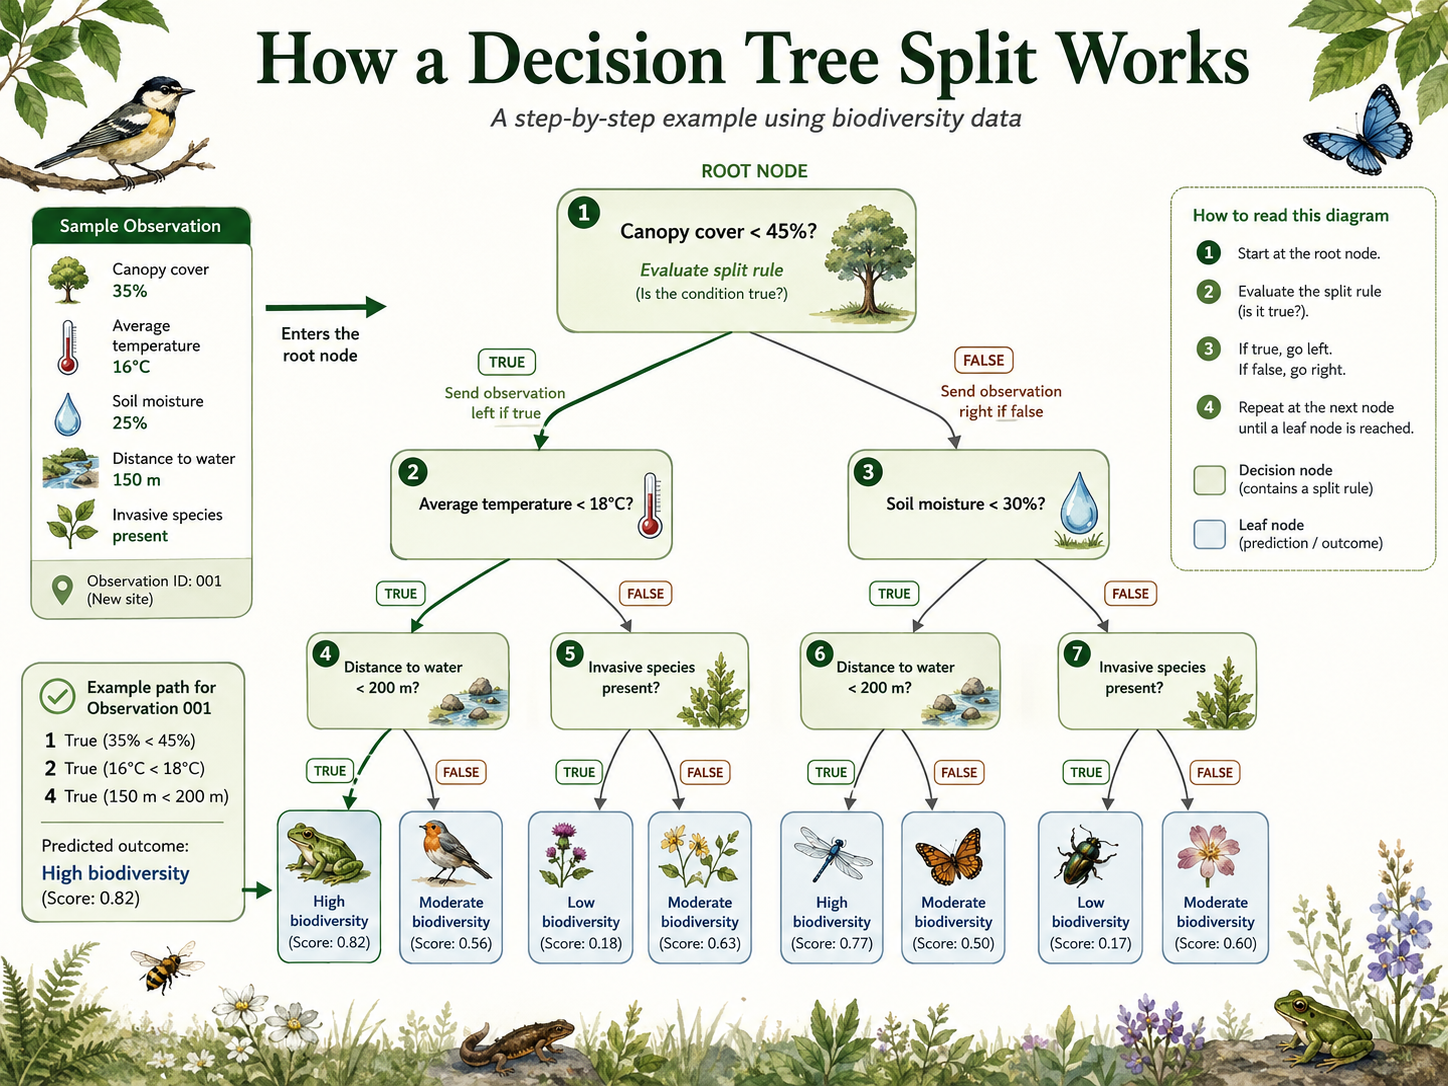
\includegraphics[width=0.8\textwidth]{Images/decision_tree.png}
    \caption{An illustrative decision tree for a regression task. The tree is built by recursively splitting the predictor space. Image generated with ChatGPT using the prompt: ``Generate an image of a decision tree that shows how a split is processed. Use a biodiversity theme for the variables.''}
    \label{fig:decision-tree}
\end{figure}

A random forest is an ensemble method that combines hundreds or thousands of decision trees to produce a prediction. Each tree is trained on a bootstrapped sample of the data, while each split considers only a random subset of the predictor variables. For regression tasks, the final prediction is obtained by averaging the predictions across all trees; for classification tasks, it is typically determined by majority vote \parencite{breiman2001, mienye_survey_2024}. This bootstrapping and aggregation, commonly referred to as bagging, also helps reduce the variance of the final model \parencite{aria_comparison_2021}.

Random forests are a popular machine learning model for top-down community-level biodiversity modeling \parencite{olaya-marin_comparison_2013, zhang2019, vecera_alpha_2019, ngor2023, cai2023, brugere2023, baggstrom2025} due to their ability to capture complex, non-linear relationships between predictors and the response variable, and their robustness to overfitting due to their ensemble nature \parencite{breiman2001}. However, some of their shortcomings include being less interpretable than GLMs and GAMs because they are an ensemble of many, possibly deep, trees \parencite{aria_comparison_2021}. Also, random forests can still show a gap between training and test performance \parencite{olaya-marin_comparison_2013, baggstrom2025}. Furthermore, they can become computationally expensive when the number of trees is large or when the depth of the trees is large.

\subsubsection{Gradient boosting}
Gradient boosting is another ensemble method but is built in a sequential manner instead of in parallel like random forests. The idea is to fit a sequence of weak learners, typically small decision trees, where each subsequent tree is trained to correct for the errors of the previous tree ensemble \parencite{friedman2001, smlbook}. The final model is an additive model of the form
\[ f_M(x) = f_0(x) + \sum_{m=1}^M \nu_m\beta_m h_m(x), \]
where \(f_0(x)\) is an initial guess, \(h_m\) is the \(m\)-th weak learner, \(\nu_m\) is the learning rate for the \(m\)-th learner, and \(\beta_m\) is the weight for that learner \parencite{friedman2001}. The model is trained in an iterative manner, where each iteration fits a new weak learner to the negative gradient of the loss function with respect to the current model's predictions \parencite{friedman2001}. Mathematically, this is expressed as 
\[r_{im} = -\left[\frac{\partial\mathcal{L}({y_i}, f(x_i))}{\partial f(x_i)}\right]_{f = f_{m-1}},\]
where \(r_{im}\) then becomes the negative gradient for the \(i\)-th observation for the \(m\)-th weak learner \(h_m\) \parencite{friedman2001}. Another way to think of it is that the dataset for the \(m\)-th weak learner,\(h_m\), becomes \(\mathcal{D} = \{(x_i, r_{im})\}_{i=1}^n\) \parencite{smlbook}. The weak learner \(h_m\) is then trained to fit these negative gradients. Once \(h_m\) is trained, \(\beta_m\) is then used to weight the contribution of the weak learner \(h_m\), and is calculated as:
\[\beta_m = \arg\min_{\beta} \frac{1}{n}\sum_{i=1}^n \mathcal{L}(y_i, f_{m-1}(x_i) + \beta h_m(x_i)),\]
where \(n\) is the number of observations, and \(\beta_m\) is usually found through a minimization optimization such as line search \parencite{friedman2001}. If the loss function is the squared error, then the negative gradient is simply the residuals of the current model's predictions, and the weak learner is trained to fit these residuals. The general algorithm can be summarized as follows:
\begin{algorithm}[ht]
\caption{Gradient Boosting Algorithm}
\begin{algorithmic}[1]
\Require \(\mathcal{D} = \{(x_i, y_i)\}_{i=1}^n\), number of weak learners \(M\), learning rate \(\nu\)
\State Initialize the model with an initial guess: \(f_0(x)\)
\For{\(m = 1\) to \(M\)}
    \State Compute the negative gradients: \(r_{im} = -\left[\frac{\partial\mathcal{L}({y_i}, f(x_i))}{\partial f(x_i)}\right]_{f = f_{m-1}}\)
    \State Fit a weak learner \(h_m\) to the negative gradient: \(h_m = \arg\min_{h} \sum_{i=1}^n \mathcal{L}(r_{im},h_m(x_i))\)
    \State Compute the weight for the weak learner: \(\beta_m = \arg\min_{\beta} \frac{1}{n}\sum_{i=1}^n \mathcal{L}(y_i, f_{m-1}(x_i) + \beta h_m(x_i))\)
    \State Update the model: \(f_m(x) = f_{m-1}(x) + \nu \beta_m h(x)\)
\EndFor
\end{algorithmic}
\end{algorithm}

An important implementation of gradient boosting is CatBoost, which was developed to handle categorical predictors more effectively and to reduce prediction shift during training through ordered boosting to deal with prediction shift, and using oblivious trees as the weak learners. CatBoost natively handles categorical features by computing ordered target statistics for each category using only preceding observations in a random permutation. Ordered boosting addresses prediction shift, which can occur when the same data are used both to estimate target statistics or gradients and to fit the model. This is mitigated by permuting the data and training models only on the data that comes before the \(i\)-th observation in the permutation. This is not feasible in practice due to the large state space and instead is done through approximation. Oblivious trees are a special type of decision tree where the same splitting criterion is used at every level of the tree, which allows for balanced trees that are less prone to overfitting \parencite{Prokhorenkova2018}. 

Gradient boosting methods are also popular for modeling large-scale plant diversity and national-scale biodiversity modeling \parencite{cai2023, baggstrom2025}. However, gradient boosting models can be sensitive to hyper-parameters, including the learning rate, tree depth, and number of boosting iterations. If these parameters are not tuned carefully, the model may overfit the training data \parencite{friedman2001}. In addition, boosting methods can be computationally expensive when the number of weak learners \(M\) is large or when the weak learners are complex.

\subsubsection{Neural networks}
Neural networks are a flexible class of machine learning models that are widely used for many applications. Here we will discuss artificial neural networks (ANNs) and specifically feed forward neural networks (FFNNs), which are used in community-level biodiversity modeling especially more recently \parencite{andermann2022, brugere2023, cai2023}. Neural networks are composed of nodes that take in input data, apply a linear transformation, and then apply a non-linear activation function to produce an output. The nodes are organized into layers, and the output of one layer serves as the input to the next layer \parencite{bishop_pattern_2006, smlbook}. Mathematically, this can be expressed as:
\begin{equation}\label{eq:neural-network}
\begin{aligned}
\mathbf{h}_0 &= \mathbf{x}_i, \\
\mathbf{z}_l &= \mathbf{W}_l\mathbf{h}_{l-1} + \mathbf{b}_l, \\
\mathbf{h}_{l} &= \sigma_l(\mathbf{z}_l),
\quad l = 1,2,\ldots,L, \\
f_\Theta(\mathbf{x}_i) &= \mathbf{W}_{L+1}\mathbf{h}_L + \mathbf{b}_{L+1}.
\end{aligned}
\end{equation}
where \(\mathbf{x}_i\) is the input vector for the \(i\)-th observation, \(\mathbf{W}_l\) is the weight matrix, \(\mathbf{b}_l\) is the bias vector, \(\mathbf{z}_l\) is the pre-activation vector, \(\sigma_l\) is the element-wise activation function for layer \(l\), and \(\mathbf{h}_l\) is the output of layer \(l\). The dimensions of each layer are:
\[\mathbf{x}_i \in \mathbb{R}^{p},
\qquad 
\mathbf{W}_l \in \mathbb{R}^{q_l \times q_{l-1}},
\qquad 
\mathbf{b}_l \in \mathbb{R}^{q_l},
\qquad
\mathbf{h}_l \in \mathbb{R}^{q_l},
\quad l = 1,2,\ldots,L, 
\]
where \(p\) is the number of input features, \(q_0 = p\), and \(q_l\) is the hidden size of layer \(l\). The activation function \(\sigma_l\) is a non-linear function, and common choices include the rectified linear unit (ReLU), \(\sigma(x) = \max(0, x)\), and the sigmoid function, \(\sigma(x) = \frac{1}{1 + e^{-x}}\). The activation function can be different between layers, but usually the same activation function is used for all layers, such as ReLU. The output layer's dimensions are: 
\[
\mathbf{W}_{L+1} \in \mathbb{R}^{m \times q_{L}},
\qquad 
\mathbf{b}_{L+1} \in \mathbb{R}^{m},
\qquad
f_\Theta(\mathbf{x}_i) \in \mathbb{R}^m,
\]
where \(m = 1\) for regression tasks and \(m = k\) for classification tasks with \(k\) classes \parencite{smlbook, prince2023understanding}. For our purposes in this thesis, we will focus on regression tasks where \(m=1\) and the output is a scalar prediction of a community-level biodiversity metric.

The parameters of the neural network are the weights and biases \(\Theta = \{\mathbf{W}_l, \mathbf{b}_l\}_{l=1}^{L+1}\). To train a neural network we define a loss function \(\ell(y_i, f_{\Theta}(\mathbf{x}_i))\) that quantifies the discrepancy between the observed response \(y_i\) and the predicted response \(f_{\Theta}(\mathbf{x}_i)\). The parameters of the neural network are updated during training by minimizing this loss function through the backpropagation algorithm \parencite{smlbook}. In backpropagation first, we will evaluate the loss of the network given a mini-batch \(\mathcal{B}\), where \(\mathcal{B} \subset \{1,...,n\}\) denotes the indices of a mini-batch. We define \(|\mathcal{B}| = B\) as the mini-batch size, so \(\mathbf{X}_{\mathcal{B}} \in \mathbb{R}^{p \times B}\) contains the mini-batch observations as columns, and \(\mathbf{y}_{\mathcal{B}} \in \mathbb{R}^{m \times B}\) contains the corresponding responses. The mini-batch is passed through the neural network in a forward pass using the matrix form of Equations~\ref{eq:neural-network}. These matrix equations are expressed as:
\begin{equation}\label{eq:neural-network-matrix}
\begin{aligned}
\mathbf{H}_0 &= \mathbf{X}_{\mathcal{B}}, \\
\mathbf{Z}_l &= \mathbf{W}_l\mathbf{H}_{l-1} + \mathbf{b}_l\mathbf{1}_B^\top, \\
\mathbf{H}_{l} &= \sigma_l(\mathbf{Z}_l),
\quad l = 1,2,\ldots,L, \\
f_\Theta(\mathbf{X}_{\mathcal{B}}) &= \mathbf{Z}_{L+1} = \mathbf{W}_{L+1}\mathbf{H}_L + \mathbf{b}_{L+1}\mathbf{1}_B^\top.
\end{aligned}
\end{equation}
The dimensions of the matrices for each layer \(l = 1,2,\ldots,L\) are:
\[\mathbf{X}_{\mathcal{B}} \in \mathbb{R}^{p \times B},
\quad \mathbf{W}_l \in \mathbb{R}^{q_l \times q_{l-1}},
\quad \mathbf{H}_{l} \in \mathbb{R}^{q_l \times B},
\quad \mathbf{b}_l \in \mathbb{R}^{q_l \times 1},
\quad \mathbf{1}_B \in \mathbb{R}^{B \times 1},
\quad \mathbf{Z}_l \in \mathbb{R}^{q_l \times B}\]
and the output layer's dimensions are:
\[\mathbf{W}_{L+1} \in \mathbb{R}^{m \times q_L},
\quad \mathbf{b}_{L+1} \in \mathbb{R}^{m \times 1},
\quad \mathbf{Z}_{L+1} \in \mathbb{R}^{m \times B}.\] 
For the regression setting considered in this thesis, the output layer is linear. The loss for a mini-batch at time \(t\) can be expressed as the average loss across the mini-batch:

\[
\mathcal{L}_\mathcal{B}(\Theta_t; \mathbf{y}_\mathcal{B}, \mathbf{X}_\mathcal{B}) = \frac{1}{B}\sum_{i \in \mathcal{B}} \ell(y_i, f_{\Theta_t}(\mathbf{x}_i)),
\]

where \(\mathcal{L}_\mathcal{B}\) is the loss over the mini-batch \(\mathcal{B}\) and \(\Theta_t\) are the parameters at time \(t\). Then we will update the network parameters \(\Theta_t\) by taking a step in the direction of the negative gradient of the loss function with respect to the parameters. This can be expressed as

\begin{equation}\label{eq:gradient-descent}
\Theta_{t+1} = \Theta_t - \alpha \nabla_\Theta \mathcal{L}_\mathcal{B}(\Theta)\bigg|_{\Theta = \Theta_t},
\end{equation}

where \(\alpha\) is the learning rate \parencite{smlbook, prince2023understanding}. This will be repeated for several iterations. At each iteration a different mini-batch is used. Mini-batches are drawn from the training data without replacement. When all mini-batches have been used, it is called one epoch. At each epoch, the training data is reused and reshuffled to generate new mini-batches. The training process will be repeated for several epochs until the model converges or a stopping criterion is met. The updating of parameters \(\Theta\) is performed using stochastic gradient-based optimization algorithms, such as stochastic gradient descent or Adam \parencite{smlbook}.

The gradients of all the parameters \(\nabla_\Theta\mathcal{L}_\mathcal{B}(\Theta_t)\) are calculated through the backpropagation algorithm, using the mini-batch loss. Since the mini-batch batch is defined as an average loss over observations, the gradient will be the average of the gradients for each observation in the mini-batch. This is expressed as:
\[
\nabla_\Theta \mathcal{L}_\mathcal{B}(\Theta_t) = \frac{1}{B}\sum_{i \in \mathcal{B}} \nabla_\Theta \ell(y_i, f_{\Theta_t}(\mathbf{x}_i)).
\]
The backpropagation algorithm uses the chain rule of calculus to compute the gradients efficiently. We describe how the gradients of each layer \(l\) can be computed using mini-batches. Using Equations~\ref{eq:neural-network-matrix}, the output layer error for layer \(L+1\) is defined as:

\[\boldsymbol{\Delta}_{L+1} = \frac{\partial \mathcal{L}_\mathcal{B}(\Theta_t)}{\partial \mathbf{Z}_{L+1}} \in \mathbb{R}^{m \times B},\]
where each column is the error for the \(i\)-th observation in the mini-batch divided by the batch size \(B\). This \(\frac{1}{B}\) is included in \(\boldsymbol{\Delta}_{L+1}\) because we are taking the average loss \(\mathcal{L}_\mathcal{B}\) over the mini-batch.
Then, the gradients for the parameters of the output layer can be calculated as:
\[
\begin{aligned}
\frac{\partial \mathcal{L}_\mathcal{B}(\Theta_t)}{\partial \mathbf{W}_{L+1}} &=  \frac{\partial  \mathcal{L}_\mathcal{B}(\Theta_t)}{\partial \mathbf{Z}_{L+1}} \frac{\partial \mathbf{Z}_{L+1}}{\partial \mathbf{W}_{L+1}} = \boldsymbol{\Delta}_{L+1}\mathbf{H}_L^\top\\ 
\frac{\partial \mathcal{L}_\mathcal{B}(\Theta_t)}{\partial \mathbf{b}_{L+1}} &=  \frac{\partial  \mathcal{L}_\mathcal{B}(\Theta_t)}{\partial \mathbf{Z}_{L+1}} \frac{\partial \mathbf{Z}_{L+1}}{\partial \mathbf{b}_{L+1}} = \boldsymbol{\Delta}_{L+1}\mathbf{1}_B,
\end{aligned}
\]
where \(H_L^\top \in \mathbb{R}^{B \times q_L}\). To continue backpropagation to the previous layer \(L\), we can calculate the error for layer \(L\) as:
\[ 
\boldsymbol{\Delta}_L = \frac{\partial \mathcal{L}_\mathcal{B}(\Theta_t)}{\partial \mathbf{Z}_L} = \frac{\partial \mathcal{L}_\mathcal{B}(\Theta_t)}{\partial \mathbf{Z}_{L+1}} \frac{\partial \mathbf{Z}_{L+1}}{\partial \mathbf{H}_L} \frac{\partial \mathbf{H}_L}{\partial \mathbf{Z}_L} = (\mathbf{W}_{L+1}^\top\boldsymbol{\Delta}_{L+1}) \odot \sigma_L'(\mathbf{Z}_L),
\]
where \(\sigma_L'(\mathbf{Z}_L) \in \mathbb{R}^{q_L \times B}\) is the element wise derivative of the activation function for layer \(L\) evaluated at \(\mathbf{Z}_L\) and \(\odot\) denotes pointwise multiplication. The gradients for the parameters of layer \(L\) can then be calculated as
\[
\begin{aligned}
\frac{\partial \mathcal{L}_\mathcal{B}(\Theta_t)}{\partial \mathbf{W}_{L}} &= \frac{\partial \mathcal{L}_\mathcal{B}(\Theta_t)}{\partial \mathbf{Z}_{L+1}} \frac{\partial \mathbf{Z}_{L+1}}{\partial \mathbf{H}_L} \frac{\partial \mathbf{H}_L}{\partial \mathbf{Z}_L}\frac{\partial \mathbf{Z}_L}{\partial \mathbf{W}_L} = \boldsymbol{\Delta}_L\mathbf{H}_{L-1}^\top\\ 
\frac{\partial \mathcal{L}_\mathcal{B}(\Theta_t)}{\partial \mathbf{b}_{L}} &= \frac{\partial \mathcal{L}_\mathcal{B}(\Theta_t)}{\partial \mathbf{Z}_{L+1}} \frac{\partial \mathbf{Z}_{L+1}}{\partial \mathbf{H}_L} \frac{\partial \mathbf{H}_L}{\partial \mathbf{Z}_L} \frac{\partial \mathbf{Z}_L}{\partial \mathbf{b}_L} = \boldsymbol{\Delta}_L\mathbf{1}_B,
\end{aligned}
\]
where \(\mathbf{H}_{L-1}^\top \in \mathbb{R}^{B \times q_{L-1}}\). This process can be repeated for each layer \(l = L, L-1, \ldots, 1\) as:
\[
\begin{aligned}
\boldsymbol{\Delta}_l = \frac{\partial \mathcal{L}_\mathcal{B}(\Theta_t)}{\partial \mathbf{Z}_l} &= (\mathbf{W}_{l+1}^\top\boldsymbol{\Delta}_{l+1}) \odot \sigma_l'(\mathbf{Z}_l),\\
\frac{\partial \mathcal{L}_\mathcal{B}(\Theta_t)}{\partial \mathbf{W}_{l}} &= \boldsymbol{\Delta}_l\mathbf{H}_{l-1}^\top,\\
\frac{\partial \mathcal{L}_\mathcal{B}(\Theta_t)}{\partial \mathbf{b}_{l}} &= \boldsymbol{\Delta}_l\mathbf{1}_B,
\end{aligned}
\]
where \(\mathbf{H}_{l-1}^\top \in \mathbb{R}^{B \times q_{l-1}}\). This iterative process gives us the gradients for all parameters in the network which can then be updated by equation~\ref{eq:gradient-descent}. The partial derivatives here are to demonstrate the chain rule and how one arrives at the gradients for each layer conceptually, but in practice these gradients are calculated efficiently through automatic differentiation libraries such as PyTorch or TensorFlow and are actually high dimensional tensors \parencite{prince2023understanding, pytorchdocs2026}.

Neural Networks are a powerful and flexible class of models that can capture complex, non-linear relationships between predictors and the response variable. They have been used for top-down community-level biodiversity modeling in several different studies \parencite{mondal2021, andermann2022, brugere2023, cai2023, hu2025} and have shown good predictive performance. However, neural networks are widely considered ``black boxes'' as it can be very difficult to interpret these models because they are so complex \parencite{pichler2023, hu2025}. Another limitation of neural networks is that they frequently have large data requirements and can take a long time to train, especially when the network architecture is large or when the dataset is large \parencite{pichler2023}. Neural networks also cannot extrapolate well outside the range of the training data, which can be a problem for community-level biodiversity modeling when we want to make predictions in new areas or under future climate scenarios \parencite{beery2021, pichler2023}.

\subsection{Current approaches and research gaps in top-down biodiversity modeling}
Community-level biodiversity modeling can be computationally intensive and methodologically demanding because study areas can span varying spatial scales from national to continental and global extents \parencite{baggstrom2025, davis2023, hoskins2020}. Depending on the size of the study area, data availability and resolution can become issues because higher resolution data for biodiversity and environmental features typically come at the cost of lower spatial coverage \parencite{wuest2020}. Furthermore, predictor selection is non-trivial because both the choice of environmental variables \parencite{williams2012} and the spatial scale at which they are measured \parencite{mertes2018scale} can influence model performance. In addition, the taxonomic scope of the community-level biodiversity metrics can vary substantially across studies because the number of species contributing to these metrics may range from hundreds \parencite{andermann2022} to hundreds of thousands \parencite{hoskins2020}, which increases modeling complexity and complicates cross-study comparisons. 

Despite these challenges, top-down biodiversity studies demonstrate the potential of these approaches and the methodological diversity of the field. A comparison of top-down modeling studies in Table~\ref{tab:literature-summary} shows the diversity of approaches used in the literature. Across the studies summarized, frequently appearing top-down modeling approaches include random forests and neural networks, while other methods like GLMs, GAMs, and gradient boosting are not as prevalent. These models are highlighted because they are widely used in the literature and will be the models used in this thesis. However, there are many other models that can be used for top-down community-level modeling such as generalized dissimilarity modeling (GDM), used for beta diversity prediction \parencite{hoskins2020}, ensemble methods \parencite{ngor2023}, and other tree based methods such as classification and regression trees or boosted regression trees \parencite{distler2015, ngor2023}. 

Model comparison is a strength of the top-down community-level biodiversity modeling literature as studies compare several models within them using a single dataset of interest. Some of these studies are summarized in Table~\ref{tab:literature-summary}. In \cite{baggstrom2025}, the authors compared a random forest, gradient boosting, convolutional neural network, and a regression model for predicting arthropod richness across Sweden. Other studies such as \cite{cai2023} compared GLMs, GAMs, random forests, gradient boosting, and neural networks for modeling plant diversity at a global scale. In \cite{mondal2021}, the authors compared GAMs, neural networks, linear mixed models, and multivariate adaptive regression splines (MARS) for modeling fish communities in India. While each study explores a different subset of models, they all perform some form of model comparison to evaluate the performance of different models for their specific application. These model comparisons also vary in the metrics used for evaluation. Common evaluation metrics include root mean squared error (RMSE), mean absolute error (MAE), and \(R^2\), while less common metrics include mean absolute percentage error (MAPE) and area under the curve (AUC) \parencite{mondal2021, andermann2022, olaya-marin_comparison_2013, vecera_alpha_2019, cai2023, brugere2023, brun2024, baggstrom2025}. In addition to these numeric metrics, visual checks are commonly used to evaluate model performance, such as plotting the community-level biodiversity metric over the spatial domain \parencite{andermann2022, brugere2023, cai2023, brun2024, baggstrom2025}.

Across the studies, there is a trend in which non-parametric models such as random forests, gradient boosting, and neural networks tend to outperform more traditional parametric models such as GLMs and GAMs, although the best model can be influenced by the dataset, predictor set, response variable, and evaluation metric \parencite{mondal2021, cai2023, brugere2023, ngor2023, baggstrom2025}. These conclusions also depend partly on the evaluation methodology. The evaluation of these models was frequently done using random k-fold cross-validation \parencite{cai2023, brugere2023, baggstrom2025}, where the data are randomly split into \(k\) folds and the model is trained on \(k-1\) folds and tested on the remaining fold. While this is a common method to evaluate a model and is a good indicator of model performance, this method assumes the data in the training and test sets are approximately independent and identically distributed (i.i.d.) \parencite{efron_estimating_1983}. In spatial modeling, however, observations are usually spatially autocorrelated meaning nearby data points are not independent of each other \parencite{elith2009}. When data are spatially autocorrelated, the assumption of i.i.d. data does not hold as data in the training and test sets can be dependent on each other. This results in random cross-validation providing an overestimation of model performance as the data in the training and test sets can be dependent \parencite{wang2023}. To account for spatial autocorrelation other cross-validation strategies can separate groups by some criteria, usually spatial location, before generating cross-validation folds \parencite{roberts2017, valavi2019}. However, among the studies summarized in Table~\ref{tab:literature-summary}, random cross-validation appears more frequently than spatial or environmental cross-validation.

A related but less explored idea is how model performance changes under data-limited scenarios. In species distribution modeling, the effect of small dataset sizes, specifically test sets, can have a profound effect on model evaluation \parencite{collart_small_2023}. Although this issue has been discussed in species distribution modeling, it is relevant to top-down modeling approaches as biodiversity data can still be limited in certain regions or for certain taxonomic groups despite the growing availability of biodiversity data \parencite{wuest2020}. Moreover, the dataset size requirements of machine learning methods increase as the model becomes more complex and in ecology, datasets of sufficient size and quality are often the exception rather than the norm \parencite{pichler2023}. Understanding how the performance of these models changes under different dataset size scenarios is important for understanding the limitations of these models and for guiding future data collection efforts.

Together, these studies demonstrate that top-down models are a promising approach for community-level biodiversity modeling, but they are also part of a fragmented landscape. Expanding top-down community-level biodiversity modeling evaluations, comparisons, and development is an important direction for future research \parencite{ferrier2002, ferrier2006, pollock2020} as top-down modeling approaches are comparable to other strategies for predicting community-level biodiversity metrics in some studies \parencite{biber2020, distler2015}. Top-down methods can also be less computationally intensive than bottom-up approaches \parencite{biber2020} as they avoid the intermediate steps of individual species modeling which also makes them conceptually more direct in community-level modeling \parencite{ferrier2006}. A flexible pipeline that allows for efficient exploration of different biodiversity datasets, predictor variables, and top-down models would promote efficient model development, testing, and comparison.

This thesis develops and evaluates a flexible pipeline for top-down community-level biodiversity modeling. This pipeline is applied to model butterfly species richness across the United Kingdom and Ireland. This case study addresses our research questions in Section~\ref{sec:research_objectives} that are motivated by the literature review. First, we position this work alongside others by comparing the performance of different top-down models for modeling species richness, reflecting the frequent use of model comparison in the literature. Second, we explore how models perform under different cross-validation strategies, specifically random and spatial cross-validation. Third, we examine how the performance of these models changes under differing dataset size scenarios as this area remains comparatively underexplored for top-down modeling approaches.

\begin{sidewaystable}[ht]
\centering
\small
\setlength{\tabcolsep}{4pt}
\renewcommand{\arraystretch}{0.8}
\caption{Summary of studies using community-level biodiversity modeling approaches in the literature with a focus on top-down models. The table includes information on the type of diversity modeled (alpha, beta, gamma), the number of predictors used, and the types of models employed in each study. The model types include generalized linear models (GLM), generalized additive models (GAM), random forests (RF), gradient boosting (GB), neural networks (NN), generalized dissimilarity modeling (GDM), stacked species distribution model (SSDM), and other specialized methods. This summary provides an overview of the current state of community-level biodiversity modeling in the literature and highlights the diversity of approaches used to model biodiversity patterns and trends.}
\label{tab:literature-summary}
\begin{tabular}{p{0.18\textwidth} ccc c p{0.06\textwidth} p{0.06\textwidth} p{0.07\textwidth} p{0.07\textwidth} p{0.07\textwidth} p{0.06\textwidth} p{0.06\textwidth} p{0.06\textwidth}}
\toprule
\multirow{3}{*}{\textbf{Study}} 
& \multicolumn{3}{c}{\textbf{Diversity type}} 
& \multirow{3}{*}{\textbf{No. predictors}} 
& \multicolumn{8}{c}{\textbf{Model type}} \\
\cmidrule(lr){2-4} \cmidrule(lr){6-13}
& \textbf{Alpha} 
& \textbf{Beta} 
& \textbf{Gamma} 
& 
& \multicolumn{5}{c}{\textbf{Top-down}} 
& \multicolumn{1}{c}{} 
& \multicolumn{1}{c}{\textbf{Bottom-up}} 
& \multicolumn{1}{c}{} \\
\cmidrule(lr){6-10} \cmidrule(lr){11-11} \cmidrule(lr){12-12} \cmidrule(lr){13-13}
& & & & & \textbf{GLM} 
& \textbf{GAM} 
& \textbf{RF} 
& \textbf{GB} 
& \textbf{NN} 
& \textbf{GDM}
&\textbf{SSDM} 
& \textbf{Other} \\
\midrule

\cite{andermann2022}
& \checkmark 
& \checkmark 
& \checkmark 
& 27 
& 
& 
& 
& 
& \checkmark 
& 
& 
& \\

\cite{baggstrom2025}
& \checkmark 
& 
& 
& 25 
& 
& 
& \checkmark
& \checkmark
& \checkmark 
& 
& 
& Regression\\

\cite{cai2023}
& \checkmark 
& 
& 
& 25
& \checkmark
& \checkmark 
& \checkmark
& \checkmark
& \checkmark 
& 
& 
& \\

\cite{brun2024}
& \checkmark 
& 
& 
& 18 
&  
& 
& 
& 
& \checkmark
& 
& \checkmark
& \\

\cite{brugere2023}
& \checkmark 
& 
& 
& 20 
& \checkmark
& 
& \checkmark
& 
& \checkmark
& 
& 
& GRNN \\

\cite{hoskins2020}
& 
& \checkmark 
& 
& 15 
&  
& 
& 
& 
& 
& \checkmark 
& 
& \\

\cite{mondal2021}
& \checkmark 
& 
& 
& 8 
&  
& \checkmark 
& 
& 
& \checkmark 
& 
& 
& (LMM, MARS)\\

\cite{ngor2023}
& \checkmark 
& 
& 
& 14 
& \checkmark
& 
& \checkmark
& 
& \checkmark
& 
& 
& (kNN, SVM, CART, Ensemble)\\

\cite{olaya-marin_comparison_2013}
& \checkmark 
& 
& 
& 7,5 
&  
& 
& \checkmark 
& 
& \checkmark 
& 
& 
& \\

\cite{vecera_alpha_2019}
& \checkmark 
& 
& 
& 19 
&  
& 
& \checkmark 
& 
& 
& 
& 
& JSDM\\

\cite{distler2015}
& \checkmark 
& 
& 
& 17 
&  
& 
& 
& 
& 
&  
& \checkmark 
& Boosted Regression Tree\\

\cite{biber2020}
& \checkmark 
& 
& 
& 8 
& 
& \checkmark
& 
& 
& 
& 
& \checkmark 
& GCM\\


\bottomrule
\end{tabular}
\end{sidewaystable}

\FloatBarrier



% \subsubsection{Bottom-up Strategy}
% The bottom-up strategy is predominately focused on predicting the distribution of an individual species through presence-only, presence-absence data, or abundance data and most often predicted with a SDM \parencite{elith2009, elith2011,waldock2022, ozkan_tumer_two_2026}. For presence-only and presence-absence data the response variable or output is a prediction for the precense or absence of a species at a given site \parencite{beery2021}. In our problem formulation, \(y_i \in \{0,1\}\) where 0 represents an absence and 1 represents a presence of the species at site \(r_i\). Importantly, a SDM predicts the presence or absence of a single species, but for community-level biodiversity metrics we need more than just one species. Therefore, our problem formulation expands to include multiple species \(S = \{s_1, s_2, \ldots, s_m\}\), where \(m\) is the number of unique species observed across the region \(R\). For each site \(r_i \in R\) and each species \(s_j \in S\) let the response variable or output be \(y_{ij}\) and it is defined as
% \[y_{ij} = \begin{cases} 
%     1 & \text{if species } s_j \text{ is present at site } r_i, \\ 
%     0 & \text{otherwise}. \end{cases}\]
% We represent all \(y_{ij}\) for site \(r_i\) as a vector \(\mathbf{y}_i = (y_{i1}, y_{i2}, \ldots, y_{im})\).
% The dataset can be represented as 
% \[\mathcal{D} = \{(r_i,\mathbf{y}_i)\}_{i=1}^n.\] 
% The transformation of \(h(r_i)\) stays the same as before, and the predictor variables are still represented as \(x_i\), so our dataset after the transformation \(h(\cdot)\) is
% \[\mathcal{D} = \{(x_i,\mathbf{y}_i)\}_{i=1}^n.\] 
% However, we will now have \(m\) models, one for each species. Therefore, the model for species \(s_j\) is
% \[f_{\Theta_j} : X \rightarrow \{0,1\}.\]
% The predicted value for species \(s_j\) at site \(r_i\) the becomes
% \[\hat{y}_{ij} = f_{\Theta_j}(x_i) = f_{\Theta_j}(h(r_i)).\]
% Species richness prediction at site \(r_i\) can then be calculated by aggregating the predicted presence of each species at site \(r_i\). A common way to do this is to sum the predicted presence of each species at site \(r_i\) \parencite{grenie2020}. This results in the following formula for species richness prediction at site \(r_i\):
% \begin{equation}
% \widehat{SR}_{r_i} = \sum_{j=1}^m \hat{y}_{ij}
% \label{eq:bottom-up-species-richness-prediction}
% \end{equation}

% Likewise, if we have abundance data, then the response variable or output is a prediction for the abundance of a species at a given site \(r_i\) \parencite{beery2021}. In our problem formulation, \(y_{ij} \in \mathbb{N}\) where \(y_{ij}\) represents the abundance of species \(s_j\) at site \(r_i\). The model for species \(s_j\) is then
% \[f_{\Theta_j} : X \rightarrow \mathbb{N}.\]
% Absolute abundance prediction at site \(r_i\) can then be calculated by aggregated the predicted abundance of each species at site \(r_i\) 
% \begin{equation}
% \widehat{A}_{r_i} = \sum_{j=1}^m \hat{y}_{ij}.
% \label{eq:bottom-up-absolute-abundance-prediction}
% \end{equation}

% While individual species predictions can be quite accurate \parencite{valavi2022} there are several challenges to bottom-up approachs. Rare species are hard to account for due to a lack of data\parencite{ferrier2006, norberg2019, zhang2020}, even though they are important to the functionailty of an ecosystem \parencite{gascon2015} excluding rare species from the analysis would therefore be problematic. Additionally, several problems arise when deciding a threshold value to determine a species presence or absence \parencite{liu_selecting_2005, distler2015}, and the method of how you stack the individual SDMs also poses challenges \parencite{biber2020}. The discussion of these challenges is beyond the scope of this, but they highlight the limitations of the bottom-up approach and the additional methodological decisions that are required for community-level biodiversity assessment.

% \subsubsection{Joint Strategy}

% Assemble and predict together approaches, on the other hand, model multiple species at once using environmental variables while accounting for biotic interactions \parencite{wilkinson2019}. The response variable or output of these approaches is a community matrix, dissimilarity matrix, correlation matrix \parencite{warton2015, nieto2018}. If the model 

% which can then be aggregated to estimate biodiversity metrics. This is most similar to a classification problem; whereas, The top-down strategy, on the other hand, is focused on predicting biodiversity metrics directly without predicting specific species which is more similar to a regression problem \parencite{pollock2020}.
% The bottom-up and predict and assemble together strategies are focused on predicting the distribution of individual or multiple species mainly through presence-only or presence-absence data \parencite{elith2009, elith2011, wilkinson2019, ozkan_tumer_two_2026}. The output of these strategies is a prediction for each species at a given site or a community matrix \parencite{nieto2018, beery2021}. which can then be aggregated to estimate biodiversity metrics. This is most similar to a classification problem; whereas, The top-down strategy, on the other hand, is focused on predicting biodiversity metrics directly without predicting specific species which is more similar to a regression problem \parencite{pollock2020}.




% The SDMs and JSDMs are focused on predicting the distribution of individual species through presence or absence data \parencite{elith2009, ozkan_tumer_two_2026}. While these models are also capable of predicting abundance data, this area is underdeveloped \parencite{waldock2022}. Even with the ability to predict abundance data, SDMs and JSDMs are still focused on predicting the distribution of individual species through presence/absence or abundance at a specific site. This would inherently imply that SDMs and JSDMs are classification problems \parencite{beery2021,valavi2022, hu2025}. This is done in SDMs by stacking several independent SDMs together and then use the aggregation to predict biodiversity metrics \parencite{ferrier2006}. JSDMs, on the other hand, model multiple species at once using environmental variables and species interactions \parencite{warton2015}. This would imply JSDMs are a multi-label classification problem. 
%add math notation here?

%should I say something about how regression models are also common in SDMs but the main point is they are classifying if a species is present or absent at a specific site. They can model a distribution at a site but the interpretation of what that actually means is unsure. When it comes down to it you are classifying if a species is present or absent at a specific site.



% more in depth on SDMs and why we move beyond them
% Species Distribution Models (SDMs) are a class of models that predict the occurrence (presence or absence) or abundance of individual species at unique geographic locations. SDMs utilize a wide range of variables such as temperature, precipitation, land cover, and human presence to make predictions on the distribution of individual species by establishing relationships between these variables and species occurrences \parencite{beery2021}. While the first SDMs were developed in the early 20th century with distributions of the Chestnut-backed Chickadee \parencite{grinnell_1904}, the application of these models has been extended beyond just generating range maps \parencite{beery2021}. They now encompass the pursuit of insights into the causal drivers of species distributions, land use management planning, conservation planning \parencite{elith2009}, revealing biological patterns, and even helping with the discovery of sites for the reintroduction of threatened species \parencite{sinclair2010}. The versatility of these models has led to their widespread use in ecology and conservation biology especially in the past few decades.

% The utility of SDMs was first expanded by the development of the Generalized Linear Model (GLM) and Generalized Additive Model (GAM) frameworks in the late 1970s and 1980s. Before these developments SDMs were primarily ecological models based on conceptual or expert knowledge of species distributions. One of the largest challenges of statistical SDMs models was the assumption of Gaussian error distributions for linear models. This assumption is often violated in ecological data. For example, count data follow a Poisson distribution \parencite{guisan2002}. The main breakthrough was first with GLMs. GLMs are able to model non-Gaussian-distributed data; specifically, any distribution in the exponential family can be modeled with a GLM \parencite{nelder1972}. GAMs then further extended the capabilities of GLMs by allowing for nonlinear relationships between the predictors and the response variable \parencite{hastie1986}. However, even with the advance of GLMs and GAMs to model non-Gaussian data and nonlinear relationships, SDMs still would struggle when there would be a dependency structure in the data and violated independent and identically distribution (i.i.d.) assumptions d\parencite{guisan2002,beery2021}. To address these issues and the need to model more complex relationships machine learning models including random forests, boosted regression trees, gradient boosting, neural networks, and ensemble methods have been increasingly used \parencite{norberg2019, beery2021,valavi2022, waldock2022, ozkan_tumer_two_2026}. These methods can capture complex nonlinear relationships and interactions between predictors and the response variable, and they can handle large datasets with many predictor variables.

% Concurrently, large advancements in the organization and distribution of biodiversity data through organizations such as the Global Biodiversity Information Facility (GBIF)\footnote{Global Biodiversity Information Facility (GBIF). Available at: \url{https://www.gbif.org/} (Accessed: 19 April 2026).} and national databases has reduced barriers to data access \parencite{ozkan_tumer_two_2026}. In addition to open biodiversity datasets, the quality of biodiversity datasets has continued to improve the quality of species data \parencite{araujo2019}. Moreover, advancements in geographical information systems (GIS) have allowed for the integration of spatial data into SDMs. This spatial data can be of climatic, environmental, topographic, or anthropogenic nature across larger areas and finer temporal scales \parencite{elith2009, waltari2014, ozkan_tumer_two_2026}. These advancements alongside with the development of new modeling techniques have further driven the advancement of SDMs with dozens of models being developed across hundreds of papers in the past few decades \parencite{valavi2022, ozkan_tumer_two_2026}.

% SDMs have been the dominant modeling family for species prediction for several decades and have been widely used in ecology and conservation biology and for good reason. They excel at predicting the distribution of individual species and contribute to our understanding of species niches \parencite{sinclair2010}. However, they are not without their shortcomings. Firstly, and the most obvious when it comes to measuring biodiversity is that SDMs are designed to predict the distribution of individual species \parencite{ferrier2006}, and most SDMs do not capture biotic interactions between species, which can be a critical driver of species distributions and community composition \parencite{waldock2022}. If we want to derive biodiversity metrics from SDMs, we would have to fit a separate SDM for each species and then aggregate the results together in a "predict first, assemble later" or bottom-up approach. This can be in itself can be very time-consuming not only to building the models themselves but also to gather all the species data and environmental data across spatial and temporal scales \parencite{ferrier2006}. Compounding this issue is the fact that most species data is still presence only data which would make biodiversity metric calculations aside from species richness difficult \parencite{valavi2022}.

% Furthermore, all SDMs are not created equally in varying environmental contexts. In some contexts such as measuring abundance, a random forest may be the best model \parencite{waldock2022}, while in a presence only context an ensemble based model may be the best \parencite{valavi2022}. Other studies have found large variations in model performance and one model may not rule them all and that the best model can vary across species and contexts \parencite{norberg2019}. This is further exacerbated by the fact that hyperparameter tuning or parameterization and feature selection models can also have a large effect on the model performance \parencite{araujo2006, beery2021}. So, if we wanted to use SDMs to predict biodiversity metrics, not only would we have to fit a separate SDM for each species but it is likely we would have to fit multiple models, and even multiple versions of the same model, for each species to find the best model for each species. SDMs also struggle to predict rare or infrequent species which can account for a large portion of species richness metrics \parencite{ferrier2006, norberg2019}. Many studies also note how transferability or extrapolation to unsampled sites is a common challenge for SDMs and is in part due to autocorrelation of environmental and spatial variables \parencite{norberg2019, a_leeyaw_species_2022}. Finally, SDMs tend to be biased at the extremes of abundance distributions, frequently overestimating low-abundance sites while underestimating sites with high abundance \parencite{waldock2022}.

% We can see that SDMs have advanced from ecological models based on expert knowledge \parencite{grinnell_1904}, to parametric statistical models \parencite{guisan2002}, to machine learning models \parencite{ozkan_tumer_two_2026}. The advancement of SDMs has concurrently been driven by advancements in quality of species data as a response variable and \parencite{araujo2019}, environmental data as predictor variables \parencite{beery2021}. SDMs can do well when it comes to prediction occurrences of individual species \parencite{a_leeyaw_species_2022}; however, the shortcomings of SDMs as a model family when it comes to modeling biodiversity metrics are significant. While aggregating multiple SDMs can be used to predict biodiversity metrics, other methods such as joint SDMs (JSMDs) have shown to be more effective at predicting biodiversity metrics \parencite{norberg2019}.

